\section{Preliminaries}
\label{sec:prelim}

In this section some background knowledge will be presented in order to understand our work. 

% NOTE: This is 1000% obvious.
%For a detailed explaination the interested reader is suggested to have a look at the cited papers. 

\subsection{Declarative Programming}
The guiding principle of declarative programming is
\begin{center} 
  ALGORITHM = LOGIC + CONTROL.
\end{center}
The idea is that the programmer should only focus on representing the problem without taking care of how to compute the solution of it. Indeed, the latter should be the job of the solver. As an example, a simple logic program \(P_1\) that  is able to append two list and to compute correctly the reversion of a list can be: 
\begin{align}
P_1 \colon \quad%
&append ([], X, X). \\
&append ([X|Y], Z, [X|T ]) \leftarrow append (Y, Z, T ). \\
&reverse([ ], [ ]).\\
&reverse([X|Y ], Z) \leftarrow append (U, [X], Z), reverse(Y, U ). \label{eq:1} \\
\intertext{
where \([\cdot|\cdot]\) is a list constructor.
If we wrote the following rule:}
&reverse([X|Y ], Z) \leftarrow reverse(Y, U ), append(U, [X], Z). \label{eq:2}
\end{align}

instead of the rule~\eqref{eq:1} in program \(P_1\), the meaning of the rule would not change and as a consequence, both programs should have the same behaviour. 

It is desirable that
\begin{enumerate}
\item the order of program rules does not matter
\item the order of subgoals in a rule body does not matter.
\end{enumerate}

\subsection{Stable Model Semantics}
% !!!!! CITATION MISSING BIG TIME !!!!!!
Research on the declarative semantics of negation in logic programming was motivated by the fact that the behavior of SLDNF-resolution \cite{}, adopted by Prolog,  does not fully match the models of programs like \(P_2\):
\begin{align}
  P_2 \colon \quad
&\mathit{pig}((88,34)). \\
&\mathit{easy\_target}(X) \leftarrow pig(X), \text{ not}\: \mathit{hard\_target}(X). \label{eq:3}\\ 
&\mathit{hard\_target}(X) \leftarrow pig(X), \text{ not}\: \mathit{easy\_target}(X). \label{eq:4}
\end{align}
Indeed, SLDNF-resolution will not always terminate when run with this program: For example, given the initial query \(\mathit{easy\_target}(pig((88,34)))\), it is necessary to prove \(\mathit{hard\_target}(pig((88,34)))\) and to so, it is again necessary to prove \(\mathit{easy\_target}(pig((88,34))\) which leads to an obvious cycle.
The non-termination for the Prolog program \(P_2\) with this query does not mean that there is no solution for it. The intuitive models for \(P_2\) are \(\{pig((88,34)), \mathit{hard\_target}((88,34))\}\) or \(\{pig((88,34)), \mathit{easy\_target}((88,34))\}\).

% !!!! WE NEED A CITATION FOR THE STABLE MODEL SEMANTICS HERE !!!! Probably Gelfond and Lifschitz?
\emph{Stable models} of a logic program \(P\) are models of \(P\) which enjoy additional properties according to natural intuitions.
Indeed stable models help us to find the intuitive model of the modified program \(P_1\) and \(P_2\). The idea is guessing an interpretation of the program, and testing its satisfiability. In order to do so, the program from which the model is wanted to be found is first reduced. 

% !!!! WE NEED A CITATION FOR THE REDUCTION !!!!!!
The algorithm for program reduction is:

Given a program \(P\) and an interpretation \(M\), its \emph{reduct} \(P^M\) is a program obtained by 
\begin{enumerate} 
\item removing rules with \(\text{not } a\) in the body for each \(a \in M\)
\item removing literals \(\text{not } a\) from all other rules % for each \(a \notin M\)
\end{enumerate}
After the reduction the least model \(LM(P^M)\) of \(P^M\) is computed and it is tested if \(M = lm(P^M)\). If the equality holds M is called a stable model of \(P\).

If we consider again the program \(P_2\), we could have the following reasonable interpretations.
\begin{align*}
M_1&= \{pig((88,34)), \mathit{easy\_target}((88,34))\}  \\
M_2&= \{pig((88,34)), \mathit{hard\_target}((88,34))\} \\
M_3&= \{pig((88,34)), \mathit{easy\_target}((88,34)), \mathit{hard\_target}((88,34))\} \\
M_4&= \{pig((88,34))\}
\end{align*}

by the definitions stated above it is easy to check that only \(M_1\) and \(M_2\) are stable models. For clarity we show that \(M_1\) is a stable model. First we reduce the program \(P_2\) to \(P_2^{M_1}\) we get the program:
\begin{align}
P_2^{M_1} \colon \quad
&pig((88,34)). \\
&\mathit{easy\_target}(X) \leftarrow pig(X). 
\end{align}
Here, rule~\eqref{eq:4} is removed since \(\mathit{easy\_target}(X) \in M_1\) and \(not\; \mathit{hard\_target}(X)\) is removed from rule~\eqref{eq:3} because \(\mathit{hard\_target}(X) \notin\; M_1\).
\subsection{Answer Set Programming}

\emph{Answer Set Programming} (ASP)~\cite{aspPrime} is a form of declarative programming 
capable of overcoming the limitations of Prolog in the programs \(P_1\) and \(P_2\).
Its high-level approach is depicted in Figure \ref{fig:ASP1} and can be summarized as follows:
\begin{enumerate}
\item Model the problem (instance) as a logic program, i.e.~in such a way that models of the logic program correspond to solutions for the problem.
\item Use an ASP system in order to compute the models of the program.
\item Extract a solution for the problem from the models of the program.
\end{enumerate}
\begin{figure}
  \caption{High-level approach of using Answer Set Programming for declarative problem solving.}
  \begin{center}
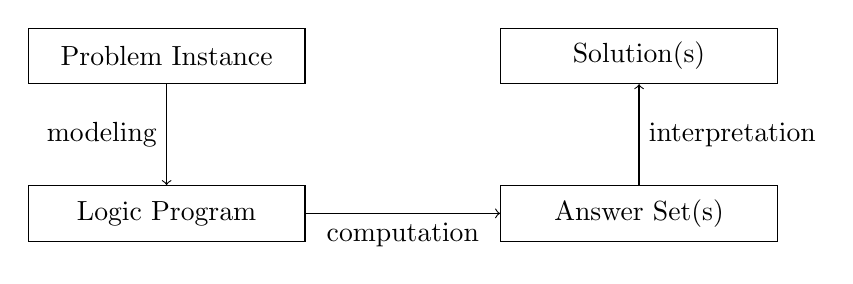
\begin{tikzpicture}
\tikzstyle{state} = [
 draw,
 minimum height=2em,
 minimum width=10em
]
\node[state] at (0,2)  (i) {Problem Instance};
\node[state] at (0,0)  (p) {Logic Program};
\node[state] at (6,0)  (r) {Answer Set(s)};
\node[state] at (6,2) (s) {Solution(s)};

\path[draw,->] (i) -> node[left]{modeling} (p);
\path[draw,->] (p) -> node[below]{computation} (r);
\path[draw,->] (r) -> node[right]{interpretation} (s);
\end{tikzpicture}
  \end{center}
  \label{fig:ASP1}
\end{figure}
 
Traditional answer set systems work in two phases:
\begin{enumerate}
\item Grounding: Given a program \(P\) with variables, a (subset) \(P'\) of its grounding is generated which has the same answer sets as \(P\).
% NOTE: Sorry, but this is just wrong on so many levels. The program actually gets exponentially bigger, and the complexity of solving it overall stays the same.
% Grounding is needed because it makes the program smaller and easier to evaluate.
\item Solving: The answer sets of the grounded (propositional) program \(P'\) are computed. First a candidate model is generated and then stability condition is checked.
\end{enumerate}

% !!!!!!!!!!!!! CITATON MISSING !!!!!!!!!!!!!!!

There are different techniques for each of the two steps described and their presentation is out of the scope of this paper. For a more detailed explanation, refer to~\cite{}.

\subsection{HEX-Programs}
HEX-programs~\cite{hex}, \emph{\underline{h}igher-order} logic programs with \emph{\underline{ex}ternal} atoms were introduced as a generalization of extended logic programs under the stable model semantics. The syntax of HEX-programs extend ordinary ASP programs by \emph{external atoms}, which enable a bidirectional interaction between a program and external sources of computation. External atoms have a list of input parameters and a list of output parameters. Informally, to evaluate an external atom, the reasoner passes the instantiated input parameters to the external source associated with the external atom. The external source computes output tuples that are matched with the output list. Formally, an external atom is of the form \(\&g[\vec{Y}](\vec{X})\), where \(\vec{Y} = Y_1, \dotso , Y_k\) are input parameters (from the set of terms, variables and predicates) and \(\vec{X} = X_1, \dotso , X_l \) are output terms.

Note that since predicate symbols may occur as input, this yields a higher order formalism. Implementations of external sources may consider the partial interpretation for input predicates at the time of evaluation.

A way to translate HEX-programs into (usual) first order programs by means of a polynomial reduction \(\Lambda(P)\) is given in \cite{hex}: (1)~Higher order atom of the form \(Y_0(Y_1, \dotso, Y_n)\) are replaced by an ordinary atom \(a_n(Y_0, Y_1, \dotso, Y_n)\). A one-to-one correspondence between stable models of \(\Lambda(P)\) and \(P\) can be shown. (2)~External atoms require a more intricate treatment. We replace external atoms of the form \(\&g[\vec{X}](\vec{Y})\) by \(p_{\&g}(\vec{X},\vec{Y})\), but in the presence of negation as failure or non-monotone external atoms, more machinery is needed which we omit for brevity. For further details on the evaluation of HEX-programs refer to \cite{effeval1,effeval2}.